%==========================================================================
%Template File for Monthly Lectual Meeting
%2006/05/22 (kkobayashi@mikilab.doshisha.ac.jp)
%==========================================================================
\documentclass[a4paper,10pt,twocolumn]{jsarticle}
\usepackage{mlm2.0}
\usepackage{epsf}
\pagestyle{plain}
\usepackage{url}
\usepackage{subfigure}
\setcounter{page}{1}
\usepackage{geometry}
\geometry{left=25mm,right=25mm,top=30mm,bottom=30mm}
%\usepackage[dvips]{graphicx}

\begin{document}
\twocolumn[
%---------------------------------------------------------------------------        % ヘッダ    書式:\beginheader{回}{年}{月}
%---------------------------------------------------------------------------
\beginheader{167}{2016}{04}
%---------------------------------------------------------------------------
% 発表題目    書式:\title{日本語}{英語} 「\\」で改行できます
%---------------------------------------------------------------------------
\title%
{git}%
%{更なる大容量化を目指して 進化しつづける次世代光メディア}

%---------------------------------------------------------------------------
% 著者名      書式:\author{日本語著者名}{英語著者名}
%---------------------------------------------------------------------------
\author{山下 俊樹,外村 篤紀\\Toshiki YAMASHITA,Atsuki TONOMURA}

%---------------------------------------------------------------------------
\endheader
%\begin{abstract}
%---------------------------------------------------------------------------
%Recently, a DVD attracts attention along with the image and the digitization of the sound. The standards of these DVD are complicated. So, in this paper, the standards of the DVD are summarized and the DVD of the next generation is refered. 
%---------------------------------------------------------------------------
%\end{abstract}
]

%---------------------------------------------------------------------------
% 本文
%---------------------------------------------------------------------------

\section{はじめに}
近年,コンピュータプログラムは大規模化し,その更新頻度は増加の一途を辿っている.そこで,コンピュータ上で作成,及び編集されるファイルの変更履歴を管理するためのバージョン管理システムが注目を集めている.現在では,かつて主流であったSVNに代わり,より高機能なgitへの移行が進んでいる.本報告では,gitの概要と関連サービスについて述べる.

\section{gitとは}
git(ギット)とは,分散バージョン管理システムの1つであり,従来用いられてきた集中バージョン管理システムに変わり登場した.その概要を以下の\fgref{git}に示す.

\begin{figure}[h]
\centering
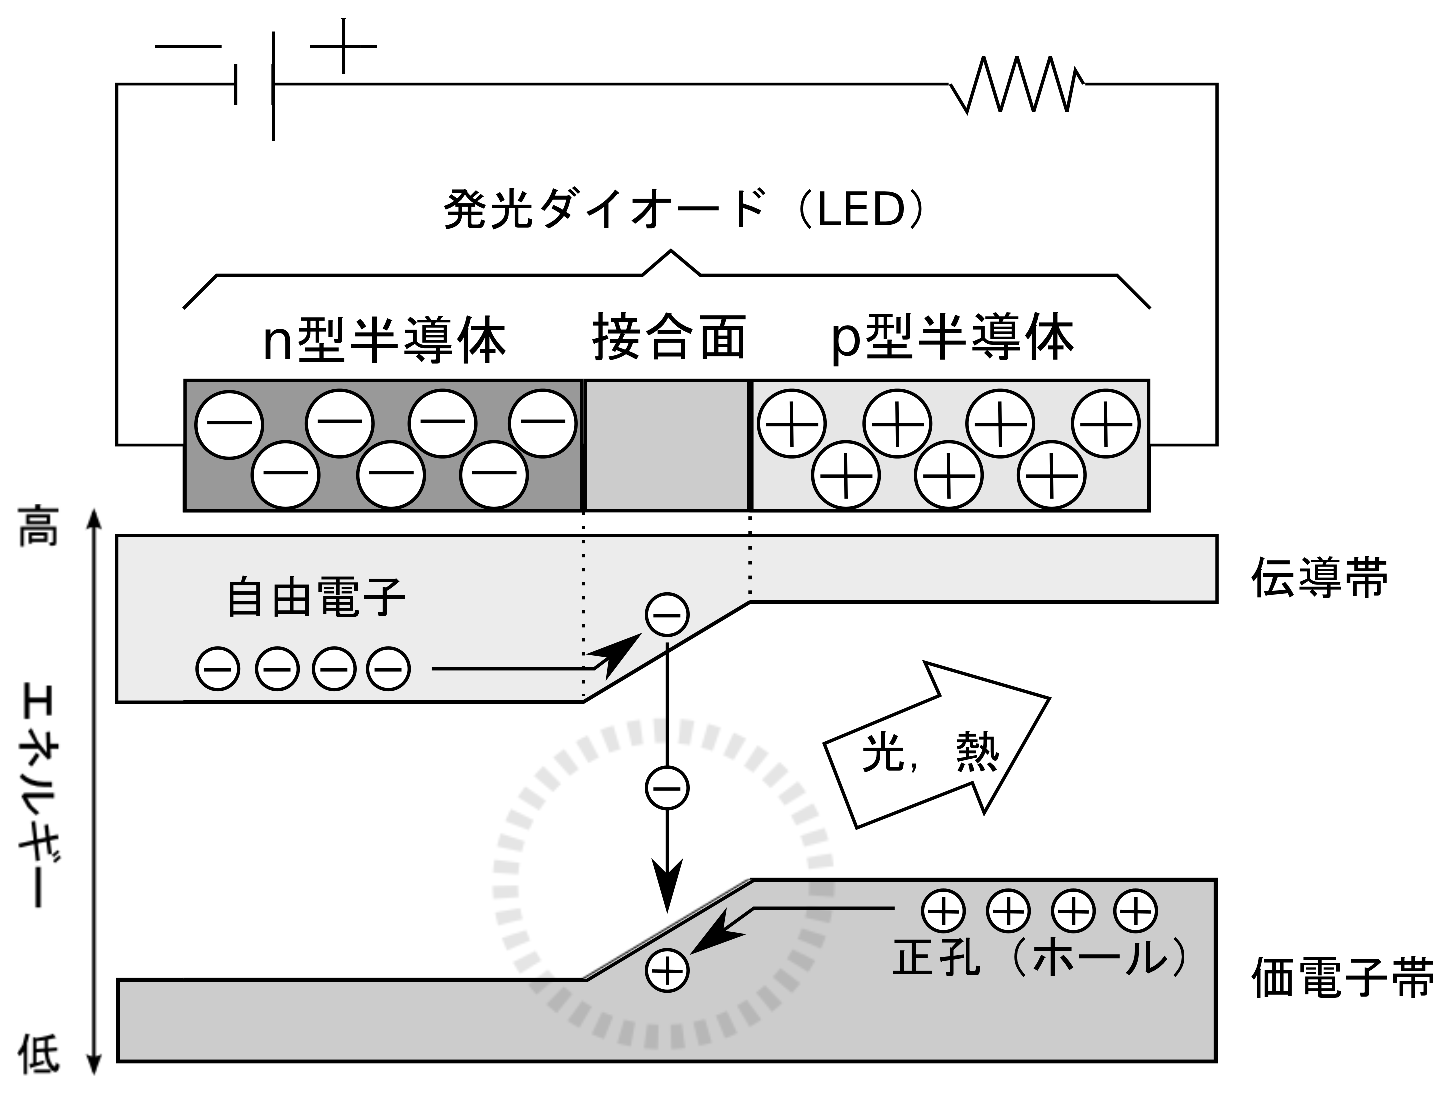
\includegraphics[width=80mm]{img/function.eps}
\caption{gitの概要}
\label{git}
\end{figure}

gitで管理されるファイルやディレクトリは,リポジトリと呼ばれる一種のデータベースにその変更が蓄積される.分散バージョン管理システムにおけるリポジトリには,サーバー上に配置され,複数ユーザーで利用するリモートリポジトリと,個人のPC内に配置され,その個人が利用するローカルリポジトリの二種類がある.ユーザーがファイル等の変更をローカルリポジトリに記録する作業をコミットと呼び,これを実行すると前回のコミットからの差分が記録される.以前のコミットの時点の状態に戻す操作及び後述するブランチを切り替える操作をチェックアウトと呼ぶ.また,ローカルリポジトリの変更をリモートリポジトリにアップロードする作業をプッシュ,リモートリポジトリからローカルリポジトリに変更をダウンロードする作業をプルと呼ぶ.

次に,gitの機能の一つであるブランチについて述べる.その一例を以下の\fgref{branch}に示す.

\begin{figure}[h]
\centering
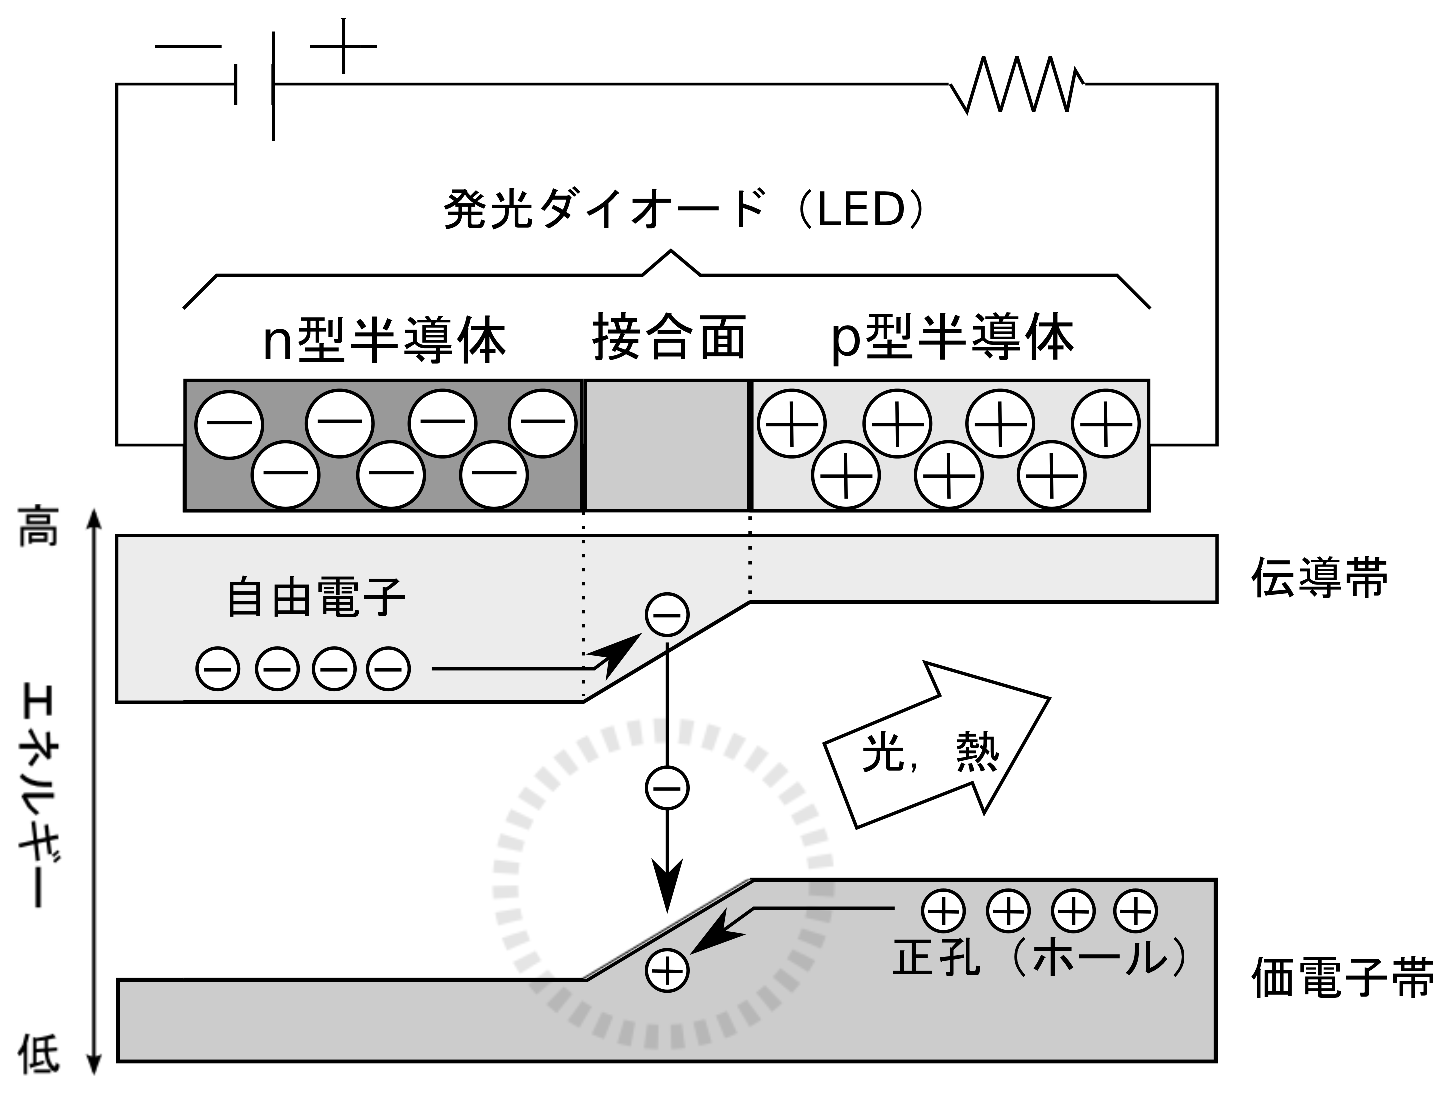
\includegraphics[width=80mm]{img/function.eps}
\caption{ブランチの一例}
\label{branch}
\end{figure}

ブランチとは,変更履歴の流れを分岐する作業と分岐後の流れを指す.また,ブランチ同士の結合をマージと呼ぶ.ブランチ同士は独立しており,他のブランチの影響を受けない.また,\fgref{branch}のように,既に運用されているソフトウエアのブランチをmasterブランチとし,そのソフトウエアのバグを修正するために用意したブランチをbugfixブランチとする.この場合二つのブランチは独立しているため,ソフトウエアの運用を止めることなくバグの修正を行うことができる.

また,他のバージョン管理ソフトウエアに対するgitの利点は次の通りである.

\begin{itemize}
\item ローカルリポジトリを持つ
\item ブランチ機能が強力
\end{itemize}

ローカルリポジトリによって,ネットワークに接続されていない環境でもコミットを行うことができる.あるいは,個人のローカルリポジトリにバグの修正のためにコミットを適量蓄積してから,リモートリポジトリにプッシュし他者に公開する等の使用方法が可能である.ブランチについては,マージを行う際に自動化されている比率が高いこと,マージが高速である等が挙げられる.

一方,欠点として,gitで扱えるのはテキストベースのファイルに限られることが挙げられる.

\section{GitHubとは}
GitHubとは,gitを利用したSNSであり,プロジェクトホスティングサービスである.ユーザーはリモートリポジトリを無料で持つことができ,他のユーザーと
コードレビュー
特徴は,フォークである
競合するサービスはBitBucket
ソーシャルコーディングの立役者
Githubは最も人気のあるgitホスティングサイトである.Olson, Rob (2008年7月22日). “GitHub unites Version Control with the Pastie”. ワシントン・ポスト 2012年1月31日閲覧


\section{今後の展望}
こんなのどうでしょう.

\small
\begin{thebibliography}{99}
\end{thebibliography}


%
%\subsection{LEDの構造と発光原理}
%\fgref{led}を参照します.
%
%\begin{figure}[h]
%\centering
%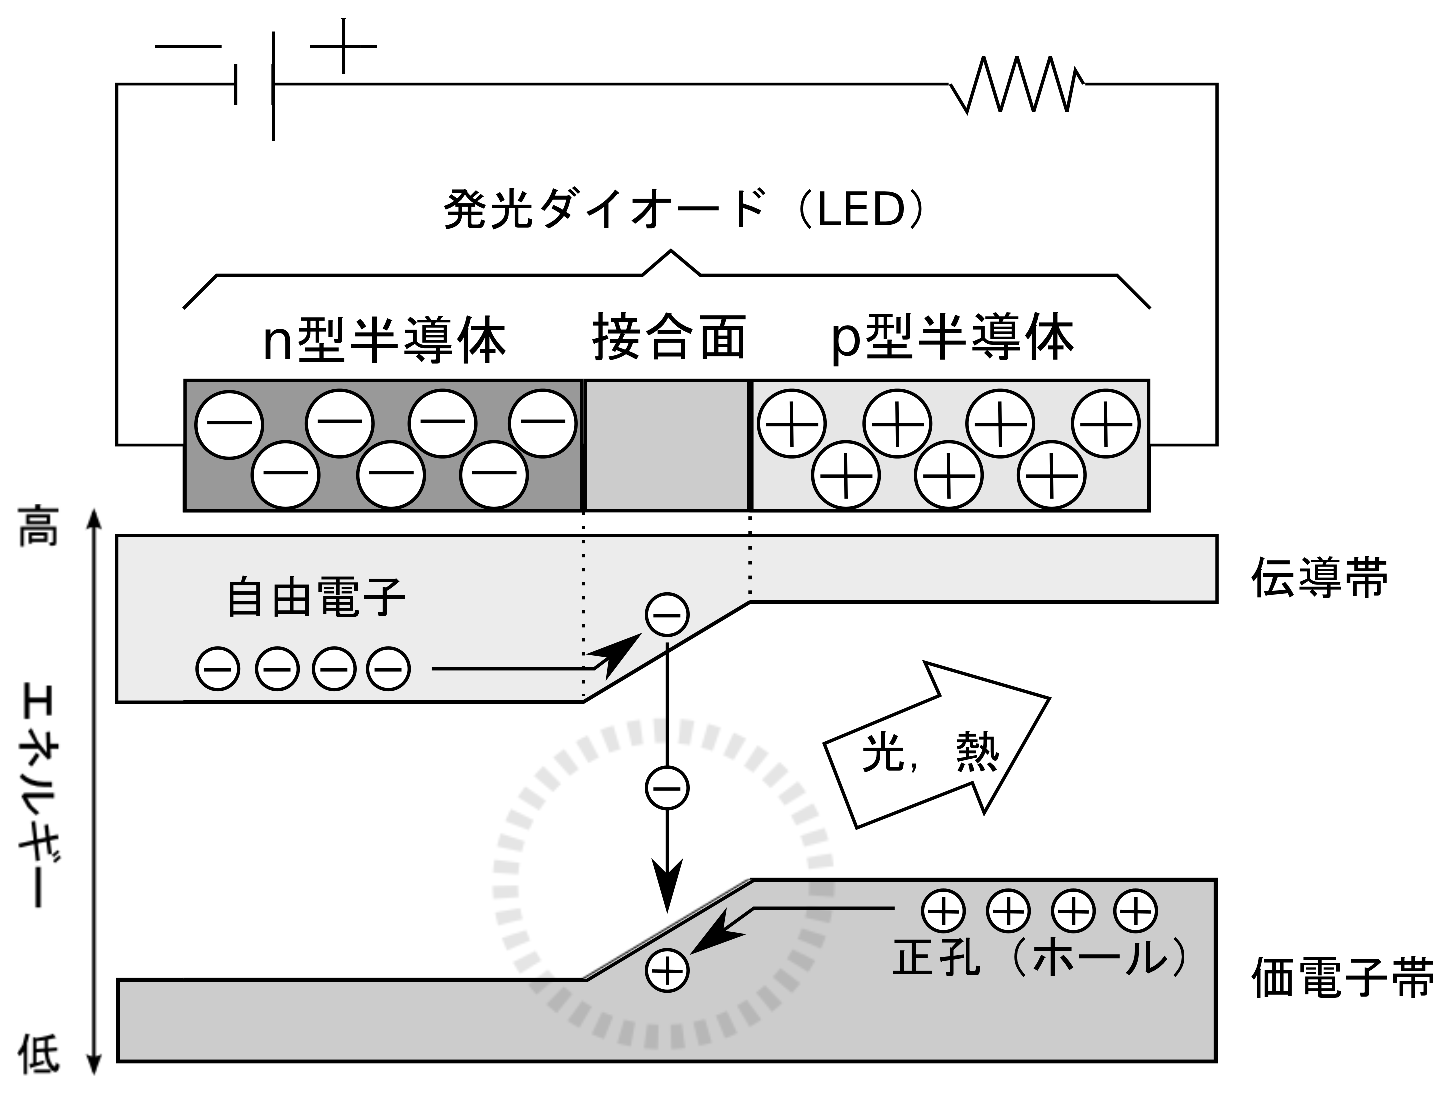
\includegraphics[width=80mm]{img/function.eps}
%\caption{参考画像1}
%\label{led}
%\end{figure}
%
%
%\fgref{sh}を参照します.
%
%\begin{figure}[h]
%
%\centering
%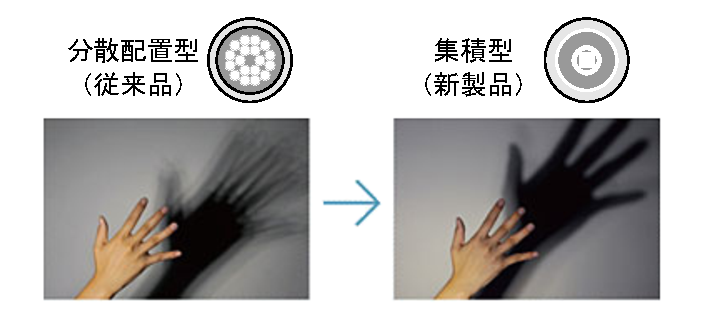
\includegraphics[width=80mm]{img/shade.eps}
%
%縦の空白を挿入する
%\vspace{3cm}
%
%
%\caption{参考画像2}
%\label{sh}
%\end{figure}
%
%
%\section{表を作る}
%
%\begin{table}[h]
%\caption{照明器具の性能比較(参考文献\cite{eru}を参照)}
%\label{table}
%\begin{tabular}{|c|l|l|l|}
%\hline
%  & 白熱電球 & 蛍光灯 & LED照明 \\ \hline
%寿命 & 1000時間 & 10000時間 & 40000時間 \\ \hline
%指向性 & なし & なし & あり\\ \hline
%発光効率 & 10 lm/W & 70 lm/W & 85 lm/W \\
% & & 〜100 lm/W & \\ \hline
%消費電力 & 54 W & 12 W & 7 W\\ \hline
%演色性 & 100 & 84 & 70〜90\\ 
%(Ra) & & & \\ \hline
%発光波長 & 赤外線が & 紫外線が & ほぼ\\
% & 多い & 多い & 可視光線のみ \\ \hline
%電源 & 交流 & 交流 & 直流 \\ \hline
%価格 & - & 白熱電球の & 白熱電球の \\
% & & 20倍 & 80倍 \\ \hline
%\end{tabular}
%\end{table}
%
%縦の空白を挿入する
%
%\tbref{table}を参照します.
%
%
%\vspace{3cm}
%
%\section{箇条書き}
%
%\begin{itemize}
%\item ユニキャスト:他にも
%\item マルチキャスト:「*」などの
%\item エニーキャスト:itemもあります
%\end{itemize}
%
%
%\begin{enumerate}
%\item ユニキャスト:このような
%\item マルチキャスト:番号付き箇条書きも
%\item エニーキャスト:可能です
%\end{enumerate}
%
%\small
%\begin{thebibliography}{99}
%
%\bibitem{SNtech}
%安藤繁,田村陽介,戸辺義人ほか:
%センサネットワーク技術-ユビキタス情報環境の構築に向けて,
%東京電機大学出版局(2005).
%
%\bibitem{reprogramming}
%Wang, Q. and Zhu, Y. and Cheng, L.:
%Reprogramming wireless sensor networks: challenges and approaches,
%{\it Network, IEEE},
%Vol.20,
%No.3,
%pp.48-55(2006).

%% -------------------

%\end{thebibliography}

%% \bibliographystyle{junsrt}
%% \bibliography{bibsample}
\end{document}
